\documentclass[a4paper, 10pt, notitlepage]{report}

\usepackage{amsfonts} % if you want blackboard bold symbols e.g. for real numbers
\usepackage{graphicx} % if you want to include jpeg or pdf pictures
\usepackage[margin=1.25in]{geometry}
\usepackage{comment}

\setlength{\parskip}{\baselineskip}%
\setlength{\parindent}{0pt}%

\title{6.830 Project: Partitioned database with deadlock detection}
\author{Benjamin Mattocks, Wenting Zheng}
\date{May 16, 2013} % change this

\begin{document}

%%%%%%%%%% PRELIMINARY MATERIAL %%%%%%%%%%
\maketitle
\thispagestyle{empty}
\newpage

%%%%%%%%%% MAIN TEXT STARTS HERE %%%%%%%%%%

\section*{Introduction}
Our project implements a distributed database with dynamic repartioning. Repartitioning is performed to reflect the database workload such that items accessed together are placed on the same server. Our project also implements distributed deadlock detection and resolution.

\section*{Data storage}
Our distributed database implements a simple key-value storage system with table support. The interface for accessing data contains the two operations \texttt{write(table\_name, key, value)} and \texttt{read(table\_name, key)}.

It also has transactional support for two-phase locking and two-phase commit. Two-phase commits are supported by an RPC protocol. Whenever a transaction is begun, a new thread is created to send and receive RPC requests used in two-phase commit.

\section*{Partitioning}
Some kind of partitioning scheme is required in a distributed database. There are several ways of approaching
this topic. The two most popular methods are hashing and range partitioning.

Range partitioning seems attractive when transactions tend to access records that are close to each other
in a table. This often happens when transactions perform a large number of range scans. However, range partitioning
requires some knowledge of the schema, and is often difficult to implement. It is also easy to get hotspots for
range partitioning.

On the other hand, hashing tends to randomize keys. This partitioning scheme is not so great for range scans
since it will most likely distribute similar keys far away from each other. However, hashing does have its advantages.
It is very easy to implement, which is the main reason why so many industrial implementations use hashing as its
partitioning method. It is also easy to scale up as the number of keys increases. 

For this project, we decided to implement a hashing-based partitioning scheme, with an adjustable number of partitions.
Based on the workload and the machine limit, the user can choose to either to have fine-grained partitioning or
coarse-grained partitioning.

\subsection*{Dynamic Re-Partitioning}

\section*{Deadlock detection}
\subsection*{Background}
A deadlock occurs when two or more process are requesting locks to items being held by other processes. More formally, it can be modeled as a Wait-For-Graph, in which a resource has a directed edge to another resource which holds a lock to an item the first resource requests. If there is a cycle in this graph, a deadlock is present.

In a distributed system, deadlock detection has been the subject of numerous studies because the distributed nature adds some complexity to the system, so certain deadlock detection algorithms might not work in a distributed environment. Distributed deadlock detection can be done with the use of centralized servers which keep track of the state of a distributed system, or they can be performed in a completely distributed manner. One problem that could occur with deadlock detection is that deadlocks might be falsely detected, which can negatively impact a system's performance. Some specific causes of this would be message delays across servers or using stale information in the WFG computed at a central server.

\section*{Implementation}
We decided to implement a fully distributed algorithm, proposed by Chandy, Misra, and Haas. This is an edge-chasing algorithm, which passes probe messages between resources directly. It is based on the AND model of deadlock detection, which implements The main idea is that the origin of the first probe knows that a deadlock is present if that probe message is received by the origin a second time. If a process is also waiting for a lock and receives a probe, it sends the probe message along to any other processes which hold locks to resources it is requesting. It retains the origin in its state so the origin will know that it sent that probe if the probe reappears there.

To implement this, we ran a specific thread for each worker on our distributed database which specifically handles these deadlock probes, independently of the main worker thread for a given transaction. This allows a worker to detect a deadlock while a specific lock is being requested. If a deadlock worker thread detects that a probe message it receives was initiated by itself, then it reports a deadlock to the worker thread and aborts the transaction. Specifically, the deadlock detection thread sets a flag in the worker thread, which then triggers an abort message to be sent by our RPC protocol to the same worker thread.

\subsection*{Test scenario}
%[figure - simple probe messages, originating at W1]
\begin{figure}[h!]

  \centering
    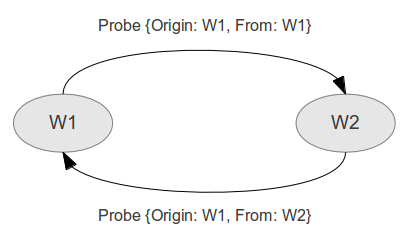
\includegraphics[scale=0.9]{deadlock-message.png}
  \caption{Probe message being propagated in network. The probe originating at W1 is sent to W2, and W2 sends the probe back to W1. W1 detects a deadlock upon arrival of the probe coming from W2.}
\end{figure}
We tested the simple case of two workers in separate threads wanting to obtain a lock held by the other concurrently. Suppose a worker W1 holds a lock on A and is attempting to get a lock on B. If a worker is attempting to lock a resource but cannot obtain the lock, a new probe message is sent to every other resource that holds a lock the worker requests. Suppose W2 holds the lock to B and wants the lock to A. If W1 first sends a probe message to W2, then W2 will send a probe message to W1 because W1 holds the lock to A, which W2 wants. W1 will receive this message and note that this message originated there, so it declares a deadlock and aborts itself.

\subsection*{Deadlock detection analysis}
Our deadlock detection scheme can detect deadlocks fairly efficiently. If there are two deadlocked transactions on two servers, this can be detected by one of the transactions in a time range between 8 and 100 ms. As the number of servers increases, the detection time should scale with the number of deadlocked transactions because only deadlocked servers communicate with each other. Compared to timeout-based methods, this can be quicker and more reliable than setting an upper bound on the time spent trying to acquire a lock. In this case, it might be waiting for a transaction to complete although it's not deadlocked.

The deadlock detector runs in a separate thread, so this can cause a performance overhead. These threads are always running when a transaction is occurring, and the threads are only utilized when a possible deadlock is happening. The number of probes from an origin is no more than the number of edges in the WFG, but there may be more probes from an origin if the deadlocks are not processed in a timely manner. We did not have a specific time requirement for deadlock detection and resolution, so deadlocks might not be resolved immediately if the process obtaining a lock is still running. We set a timeout to stop the process from trying to obtain a lock and to proceed with the abort if there is in fact a detected deadlock.

Further optimizations that could occur but that we did not implement include localized deadlock detection and reduced probe frequency. That is, if the transactions in a WFG reside in the same server, the probing would not need to occur over RPC because the WFG would be local. This could save some RPC communication overhead in the real world, and because our database repartitions data according to how often values are accessed at the same time, this could present an opportunity to implement localized detection. The probe frequency could also be decreased following some optimizations provided by Chandy et al, perhaps by probing at certain time intervals.

\section*{Analysis}

\section*{Conclusion}
We implemented a distributed database that supports repartitioning and deadlock detection.

Our database does not have support for joins. There is also no fault tolerance in our system. The two-phase commit could be extended to support logging and recovery.

\begin{comment}
%%%%%%%%%% BIBLIOGRAPHY %%%%%%%%%%
\chapter*{Bibliography}
%
\begin{description}

\item Author, I. (Year). \emph{Book Title}, Publisher; Place of publication.

\item Lamport, L. (1986), \emph{\LaTeX: A Document Preparation System}, Addison-Wesley; Reading, MA.

\item Author, I. (Year). `Journal article title', \emph{Journal}, \textbf{Vol}, pp.first--last.

\item Smith, A.D.A.C. and Wand, M.P. (2008). `Streamlined variance calculations for semiparametric
mixed models', \emph{Statistics in Medicine}, \textbf{27}, pp.435--48.

\end{description}
\end{comment}
\end{document}
